%=================================================================
% RELab LaTeX template - this template is based on the IMRT and ASL LaTeX template
%=================================================================

\documentclass[10pt,twoside,a4paper]{report}


 \usepackage{ethReLab}   	% New styles and commands

% \includeonly{}                      				% Quick formatting
% \usepackage[draft]{graphicx}        		% Quick formatting

 \usepackage{a4}                      			% Paper size
 \usepackage[latin1]{inputenc}       			% Keybord settings
 \usepackage{amsmath}                 			% Additional math functionality
 \usepackage{amssymb}                 		% Additional math functionality
 \usepackage{float}                   			% Placement of floating objects
 \usepackage{fancyhdr}                			% Headings
 \usepackage{rotating}
 \usepackage{multirow}
 \usepackage{url}
 \usepackage{colortbl}
 \usepackage{ifpdf}
\usepackage[final]{pdfpages}
\usepackage{mcode}
\usepackage{cite}


 \usepackage{hyperref}
 \usepackage{color}
 \definecolor{black}{rgb}{0,0,0}
 \definecolor{white}{rgb}{1,1,1}

 \definecolor{darkred}{rgb}{0.5,0,0}
 \definecolor{darkgreen}{rgb}{0,0.5,0}
 \definecolor{darkblue}{rgb}{0,0,0.5}

%\usepackage{german}                  		% German language
%\usepackage{ae}                      			% German specials

\usepackage{hyperref}						% generates colored links in pdf file
\hypersetup{
     		bookmarks = true,
     		colorlinks = true,       				% false: boxed links; true: colored links
    		linkcolor = black,          				% color of internal links
    		citecolor = black,        				% color of links to bibliography
    		filecolor = black,      				% color of file links
    		urlcolor = black          				% color of external links
}



%---------------------------------------------------------------------------

 \setlength{\parindent}{0em}                   		% Disable parindent
 \rhead[\thepage]{\nouppercase{\rightmark}}    % Special headings
 \lhead[\nouppercase{\leftmark}]{\thepage}     	% Special headings
 \cfoot{}                                      					% Special headings

%---------------------------------------------------------------------------

 \title{Experimental Methods For Engineers}
\subtitle{Intrusive Probe Measurement Technique In Turbomachinery}


\projecttype{Report}
% Internship Report, Bachelor-Thesis, Semester-Thesis, Master-Thesis

\studentA{Maximilian Boosfeld}
\studentB{Michel Heusser}
\studentC{Kaspar Schlegel}

\supervisionA{Sebastiano Lazzi}
%\supervisionB{Supervisor B}
%\supervisionC{Supervisor C}

\professorA{Prof. Dr. R.S. Abhari}
%\professorB{Prof. B}
%\professorC{Prof. C}

\timeperiod{October 2012}

%===========================================================================
\begin{document}

%---------------------------------------------------------------------------
% Title page

 \maketitle
 \pagestyle{plain}
 \pagenumbering{roman}

%---------------------------------------------------------------------------
% Project Description Page
%\includepdf[pages={1}]{ProjectDescription}
 %\cleardoublepage

%---------------------------------------------------------------------------
% Preamble

 %!TEX root = Report.tex
% Acknowledgment -----------------------------
%\chapter*{Acknowledgments}

%Acknowledge people who helped you and contributed to this project here \dots

 %\cleardoublepage

%---------------------------------------------------------------------------
% Table of contents

 \setcounter{tocdepth}{2}
 \tableofcontents

 %\cleardoublepage

%---------------------------------------------------------------------------
% Lists

 \listoffigures % Creates list of all figures used in document
% \cleardoublepage

 % \listoftables  % Creates list of all tables inserted
 %\cleardoublepage

%---------------------------------------------------------------------------
% Abstract

%\chapter*{Abstract}
 %\addcontentsline{toc}{chapter}{Abstract}

%---------------------------------------------------------------------------
% Symbols

%\chapter*{Symbols}\label{chap:symbole}
% \addcontentsline{toc}{chapter}{Symbols}
%
%\section*{Symbols}
%\begin{tabbing}
% \hspace*{3cm} \= \kill
%  $\phi, \theta, \psi$	\> roll, pitch and yaw angle \\[0.5ex] 					
%  $b$				\> gyroscope bias \\[0.5ex]										
%  $\Omega_m$		\> 3-axis gyroscope measurement \\[0.5ex]   		
% \end{tabbing}
%
%\section*{Indices}
%\begin{tabbing}
% \hspace*{1.6cm}  \= \kill
% $x$ \> x axis \\[0.5ex]
% $y$ \> y axis \\[0.5ex]
% \end{tabbing}
%
%\section*{Acronyms and Abbreviations}
%\begin{tabbing}
% \hspace*{1.6cm}  \= \kill
% ETH \> Eidgenoessische Technische Hochschule \\[0.5ex]
% EKF \> Extended Kalman Filter \\[0.5ex]
% IMU \> Inertial Measurement Unit \\[0.5ex]
% UAV \> Unmanned Aerial Vehicle \\[0.5ex]
% UKF \> Unscented Kalman Filter \\[0.5ex]
%\end{tabbing}
%
% \cleardoublepage

%---------------------------------------------------------------------------


 \pagestyle{headings}                 	% Default headings
 \pagestyle{fancy}                   		% Special headings
 \pagenumbering{arabic}

%---------------------------------------------------------------------------
% Chapters

 %!TEX root = Report.tex
\chapter{Introduction}\label{sec:introduction}
Schlieren photography is a powerful technique to visualize density and temperature variations in flows. It was invented 1864 by August Toepler to examine supersonic motion. Schlieren technology is based on the principle of light being bent by refractive index variations due to the different propagation speed of light. $n=\frac{c_0}{c}$ 

\section{Optical Density Measurements}
The classical Schlieren technology consists of a point source of illumination, several lenses, a test section and a camera as depicted in Figure \ref{pic:Setup_optical}. \\
\begin{figure}[H]
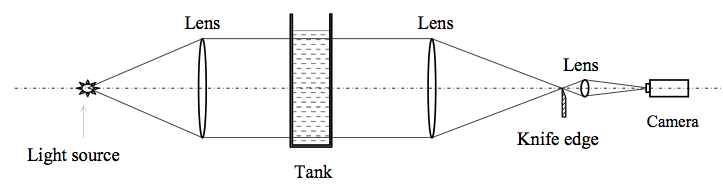
\includegraphics[width=1\textwidth]{pics/Setup_optical.png}
\caption{Working Principle Optical Schlieren - \emph{Source:} \cite{thomas2009synthetic}}
\label{pic:Setup_optical}
\end{figure}

In the test section the collimated light beam is distorted by density gradients in the fluid. Distortions create spatial variations in light intensity and the "knife" stops the rays deviated from parallelism. Though all Schlieren technologies have the huge advantage of being non-invasive there are several difficulties to this technique. First of all the experimental setup of positioning the lenses is complicated, sensitive to disturbances and fairly expensive. Furthermore the emitted light from a single-point source is limited as well as the size of lenses. Finally direct quantitative analysis remains difficult due to the fact that all information is encoded in brightness and no absolute reference is available.

\section{Schlieren measurements, Examples Of Use}

Background Oriented Schlieren (BOS), first introduced in the late 1990's, is a much simpler technique of the larger field of Synthetic Schlieren. Just as the optical Schlieren method it is commonly used for two-dimensional flow visualizations of temperature and density changes in several fields, such as fluid mechanics, ballistics, heat exchange through convection, as well as observing the propagation and mixing behavior of gases. Latest developments of this technique even allow precise quantitative visualization of fluid flows, coupling the refractive index with flow properties.

\section{Working Principle Of Synthetic Schlieren Method}

As mentioned earlier the setup for the Synthetic Schlieren technique is much simpler than one of the Optical Schlieren method. Beams from the diffuse light source pass through a mask and are captured by a digital camera as illustrated in Figure \ref{pic:Setup_synthetic}. A reference picture (without test section) is compared with one containing the test section.
\begin{figure}[H]
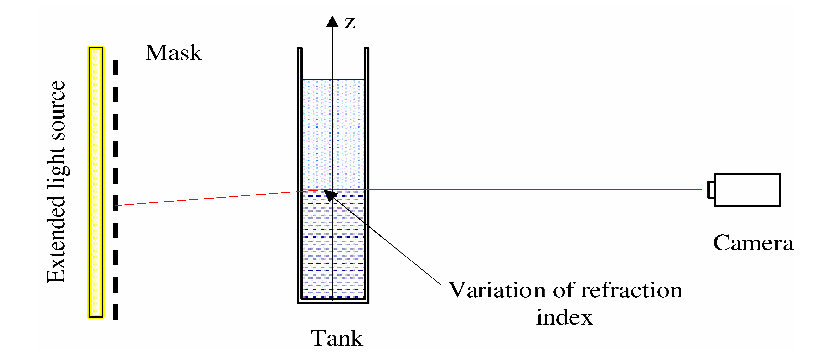
\includegraphics[width=1\textwidth]{pics/Setup_synthetic.png}
\caption{Working Principle Synthetic Schlieren - \emph{Source:} \cite{thomas2009synthetic}}
\label{pic:Setup_synthetic}
\end{figure}
The improvements are obvious. No expensive mirrors, lenses and no single-point source of light is needed. The technique of Background Oriented Schlieren (BOS) is even simpler. Instead of an extended light source and a mask only a random background pattern is needed.\\
To derive from optical distortions to temperature or density variations, a relation between refractive index and fluid properties is needed. The "Gladstone-Dale" relationship 
\begin{equation}
n-1 = K \cdot \rho = K \cdot \frac{p}{RT}
\end{equation}
provides such link for gases. The empirical relationship for paraffin oil used in the experiment is shown below.
\begin{equation}
n(T)= 1.48-0.00036 \cdot T(^\circ C)
\label{eq:nparafin}
\end{equation}


 %!TEX root = Report.tex
\chapter{Laboratory Description}\label{sec:experimentalsetup}

\section{Experimental Setup}
The experiment consists of a tank filled with warm water at $T_i=51 ^\circ C$ and a test section connected to it as shown schematic in Figure \ref{pic:schematic}. The water from the reservoir is constantly pumped through the test section so that all components should roughly be heated up to $T_i$. 
\begin{figure}[H]
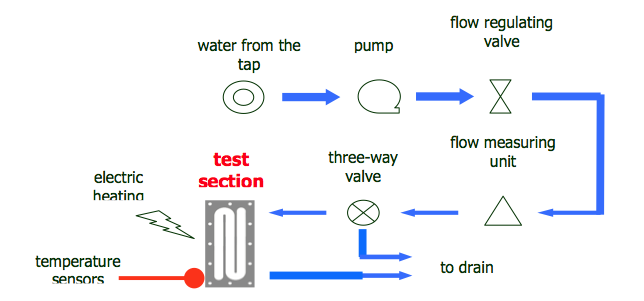
\includegraphics[width=1.0\textwidth]{pics/schematic}
\caption{Schematic Setup of the Experiment}
\label{pic:schematic}
\end{figure}
The test section itself contains an aluminum back plate with a TLC-sheet on its surface. In the cooling channel some v-shaped obstacles are arranged to cause a turbulent flow. The front plate is made out of plexiglas allowing the camera to capture pictures of the TLC-sheet.
\begin{figure}[H]
\mbox{
\subfigure[]{
\includegraphics[width=.25\textwidth]{pics/testsection1}
\label{pic:testsection1}}\quad
\subfigure[]{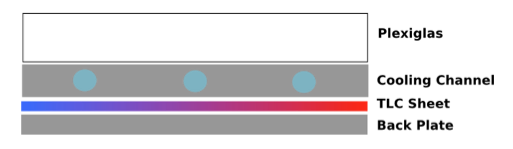
\includegraphics[width=.7\textwidth]{pics/testsection2}
\label{pic:testsection2}}}
\caption{Testsection (a) with obstacles (b) schematic}
\label{pic:testsection}
\end{figure}

\section{Experimental Procedure}
As mentioned above water is pumped through the closed loop for about an hour to obtain the uniform  temperature $T_i= 51 ^\circ C$ in all components. Measurements start as soon as the three-way valve is opened (t=0) and a cold water pulse runs through the test section at $T_\infty=10 ^\circ C$. A CCD camera linked to a computer captures the change of color of the liquid crystals foil caused by the temperature drop. A simultaneously started MATLAB file saves the camera's 100 pictures and post processes the data.

 %!TEX root = Report.tex
\chapter{Theory}\label{sec:methodofattack}

\section{Model Building}
In order to measure the local heat coefficient $\alpha$ a valid experimental model is required. To create a model which performs similar to the real heat exchange inside a blade non-dimensional characteristic numbers have to match. Although a turbine blade is internally cooled with air and the presented model uses water, a matching Reynolds number $Re=\frac{\rho v L}{\mu}$ yields in equitable flow conditions. However also Prandtl number $Pr=\frac{\nu}{\alpha}$ and Nusselt number $Nu=\frac{\alpha L}{\lambda}$ have to match in order to guarantee equal thermal conditions and conductivity. Finally another simplification is made by supposing only one-dimensional heat transfer to be relevant.
\begin{figure}[H]
\centering
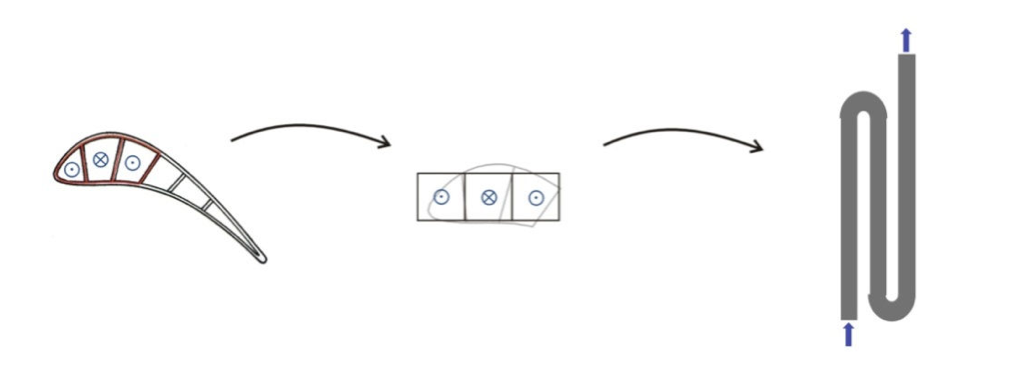
\includegraphics[width=.8\textwidth]{pics/modelbuilding}
\caption{From Blade to Experimental Model}
\label{pic:modelbuilding}
\end{figure}

\section{Heat transfer}

The heat transfer coefficient $\alpha$ is determined from the unsteady one-dimensional heat conduction equation. The assumption for one-dimensional heat transfer is valid, because we consider only a very short time period and because we have only the thickness of the Aluminium plate as relevant geometric parameter, the other dimensions are in comparison very large. The time constant is given in equation \ref{eq:timeconstant}

\begin{equation}
t_{max}=\frac{L^2}{a}=0.9983\ s
\label{eq:timeconstant}
\end{equation}

with a the thermal diffusity defined in equation \ref{eq:diffusity} and $L=10\ mm$. 

\begin{equation}
a=\frac{\lambda}{\rho c_p}=0.10016 \cdot 10^{-3}\ m^2/s
\label{eq:diffusity}
\end{equation} 

where for Aluminium $\lambda=238\ W/mK$, $\rho=2700\ kg/m^3$ and $c_p=880\ J/kg K$. \\

The basic one-dimensional conduction equation is shown in equation \ref{eq:heat1D}.

\begin{equation}
\frac{\partial T}{\partial t}=a \frac{\partial^2 T}{\partial x^2} 
\label{eq:heat1D}
\end{equation}

To solve this equation, we need to specify initial and boundary conditions as given in the following:

\begin{equation}
T(x,t=0) = T_i \nonumber
\end{equation}

\begin{equation}
T(x \rightarrow \infty,t) = T_i \nonumber
\end{equation}

\begin{equation}
\lambda \left. \frac{\partial T}{\partial x}  \right|_{x=0}=\alpha(T_{\infty}-T(0,t)) \nonumber
\end{equation}

where $T_i=51^{\circ}$ is the initial temperature and $T_{\infty}=10^{\circ}$ the fluid temperature.

The solution of the differential equation is evaluated at $ T(x=0,t)=T_s $ and can be seen in equation \ref{eq:sol}. 

\begin{equation}
\frac{T_s-T_i}{T_{\infty}-T_i}=1-\exp \left( \frac{\alpha^2 a t}{\lambda^2}\right)  \operatorname{erfc} \left( \frac{\alpha \sqrt{a t}}{\lambda} \right)
\label{eq:sol}
\end{equation}

In the measurement, we obtain the surface temerature in function of the time. As we want to determine $\alpha$, we have to solve this equation but it is not linear in $\alpha$ and can not be solved explicitely. Therfore the delivered MATLAB file calculates the solution numerically.


\section{Thermochromic Liquid Crystals (TLC)}

With the help of Thermochromic Liquid Crystals (TLC), the surface temperature is visualized. TLC react to change of temperatures by changing their colors. This substance shows properties between a crystalline solid and an isotropic liquid. \\

The long chain organic molecules are aligned in a certain direction. In order to reach a dense packing, the molecules are arranged with a slight twist. On a larger scale, this leads to a helical orientation. This helix has a pitch (distance over which  molecule rotates over $360^\circ$). Light hitting this structure is transmitted and reflected. Only the component of the light which has circular polarization with the same hand sign as the helix direction is transmitted, while all others are reflected. In consequence, when white light hits the structure, only one particular wavelength is reflected.\\

As the temperature changes, the helical structure varies. Increasing the temperature leads to two effects: thermal expansion of the helice which increases pitch and faster twist which decreases twist. The second effect is usually dominating. This results in a diminution of the molecule and a color change to shorter wavelengths.\\

In our experiment we use TLC with a temperature range from $35^\circ$C to $37^\circ$C. When the temperature is out of this range, the crystals appear black. Before the actual experiment, a calibration has to be done to allocate the different colorings to a particular temperature, which has been already done for us.




 %!TEX root = Report.tex
\chapter{Measurements And Results}\label{sec:results}

\section{Calibration process}
As mentioned above the TLC had to be calibrated. This is quiet a time-consuming procedure, because the assumptions is made that the temperature change proceeds quasi-stationary implying that after each step thermal equilibrium is reached. RGB-data from the camera is converted to HSI and after polynomial interpolation the Hue-value correlates with the temperature as shown in figure \ref{fig:calibration}.

\begin{figure}[H]
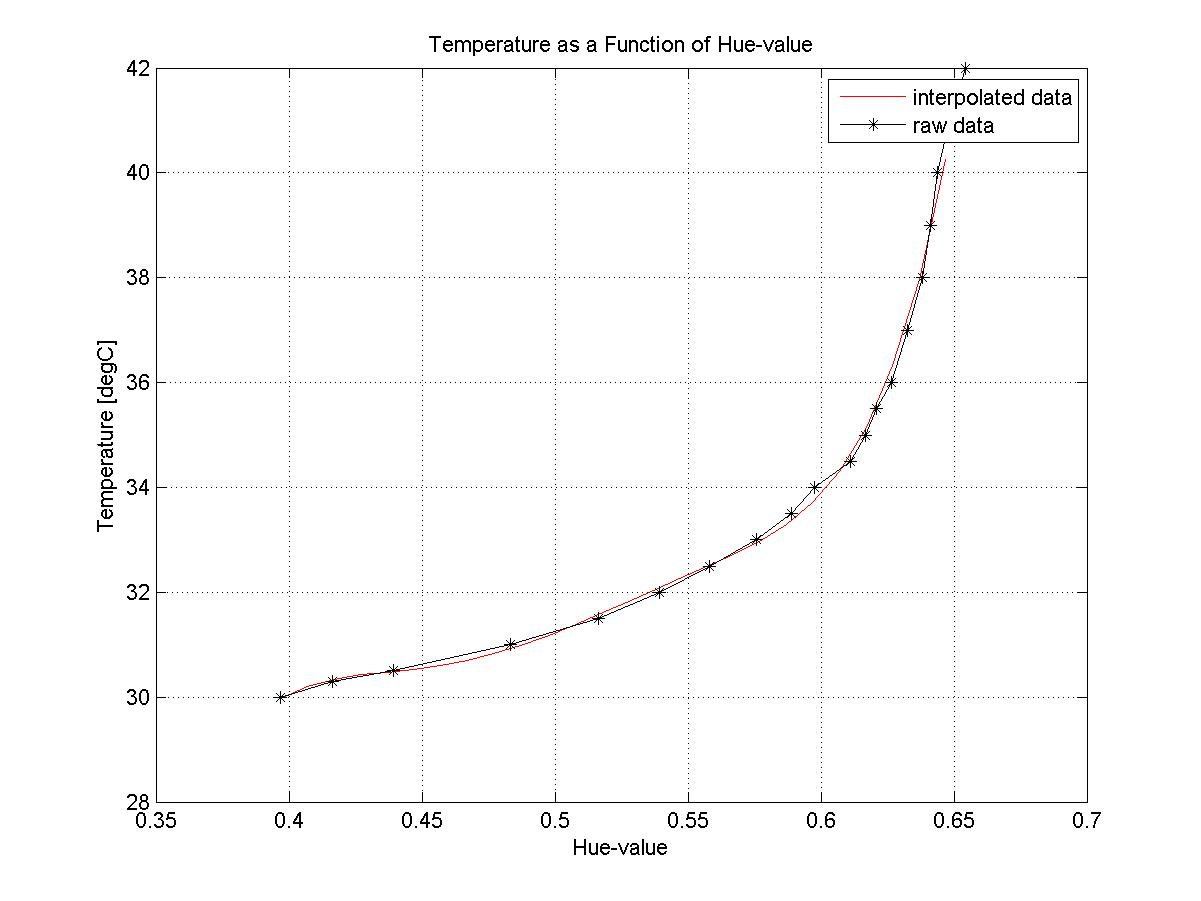
\includegraphics[width=0.95\textwidth]{pics/calibration}
\caption{Temperature as Function of Hue Value}
\label{fig:calibration}
\end{figure}


\section{Measurements}
The measurements we took did not yield to any meaningful result, because the camera didn't record the propagating front of cold water and thus no change in color was observed.
\section{Qualitatively Correct Results}
However the advisor provided us with reasonable results from a previous run of the experiment shown in figure \ref{fig:temperature} below. The camera took 100 pictures but only frame 1 to 12 depict a change in color. It seems like the cold water pulse already passed the test section and only the last part of the temperature drop is represented.
\begin{figure}[H]
\centering$
\begin{array}{cccccc}

\includegraphics[width=.14\textwidth]{pics/91} &

\includegraphics[width=.14\textwidth]{pics/92} &

\includegraphics[width=.14\textwidth]{pics/93} &

\includegraphics[width=.14\textwidth]{pics/94} &

\includegraphics[width=.14\textwidth]{pics/95} &

\includegraphics[width=.14\textwidth]{pics/96} \\

\includegraphics[width=.14\textwidth]{pics/97} &

\includegraphics[width=.14\textwidth]{pics/98} &

\includegraphics[width=.14\textwidth]{pics/99} &

\includegraphics[width=.14\textwidth]{pics/910} &

\includegraphics[width=.14\textwidth]{pics/911} &

\includegraphics[width=.14\textwidth]{pics/912} 
\end{array}$
\caption{Change of Color Picture 1 to 12}
\label{fig:temperature}
\end{figure}


Eventually the MATLAB script computed the heat transfer coefficient $\alpha$ and the surface temperature $T_s$ and plotted the values in function of time displayed in figure \ref{fig:alpha} and figure \ref{fig:surfaceT}. Apparently initial conditions for the computation are defined wrong yielding to very high values of $\alpha$ and very low temperatures at the beginning of the experiment. Between $t=0.4\ s$ and $t=2\ s$ an exponential temperature decline is observed. Furthermore the heat coefficient goes up and down although it should be constant yielding in a rough average of $\alpha = 8\ kW/m^2K$.

\begin{figure}[H]
\mbox{
\subfigure[]{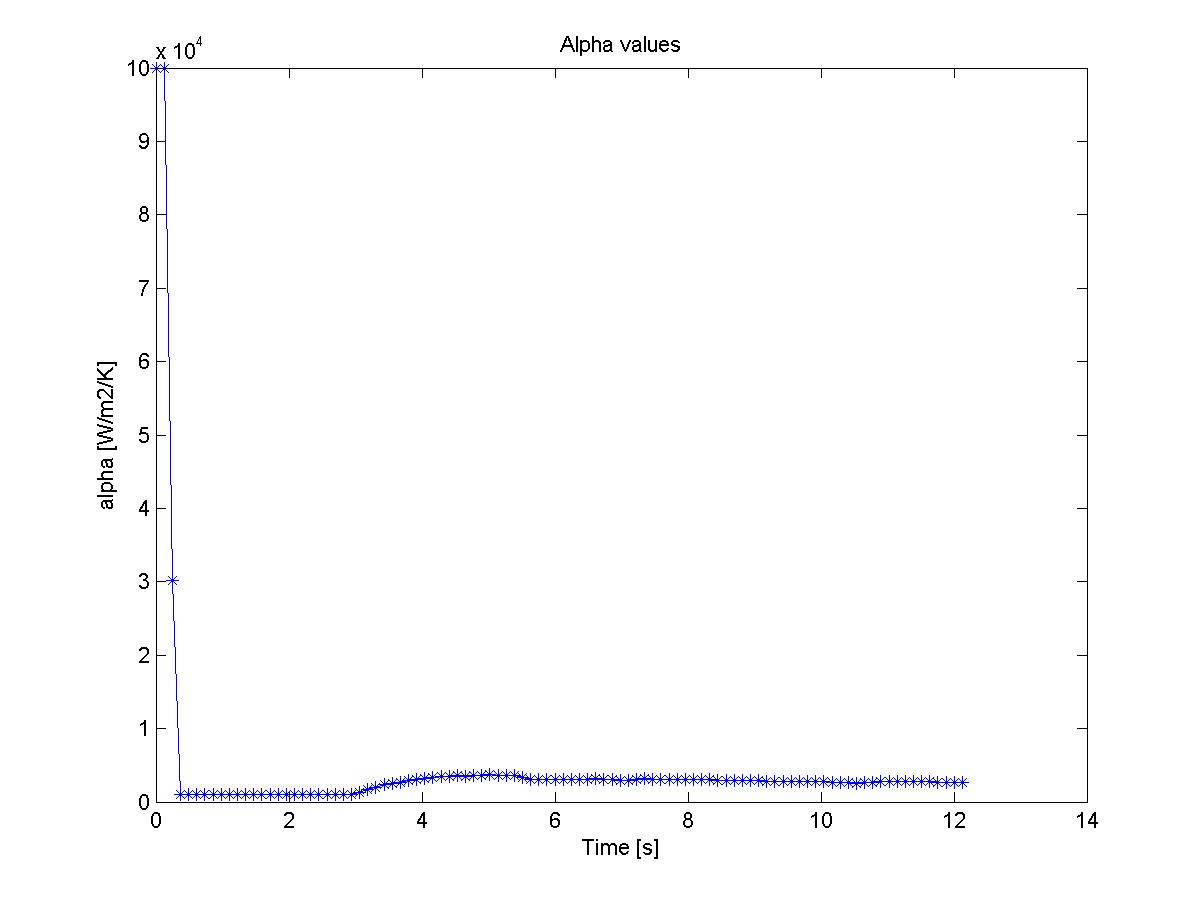
\includegraphics[width=.5\textwidth]{pics/alpha}
\label{fig:alpha}}\quad
\subfigure[]{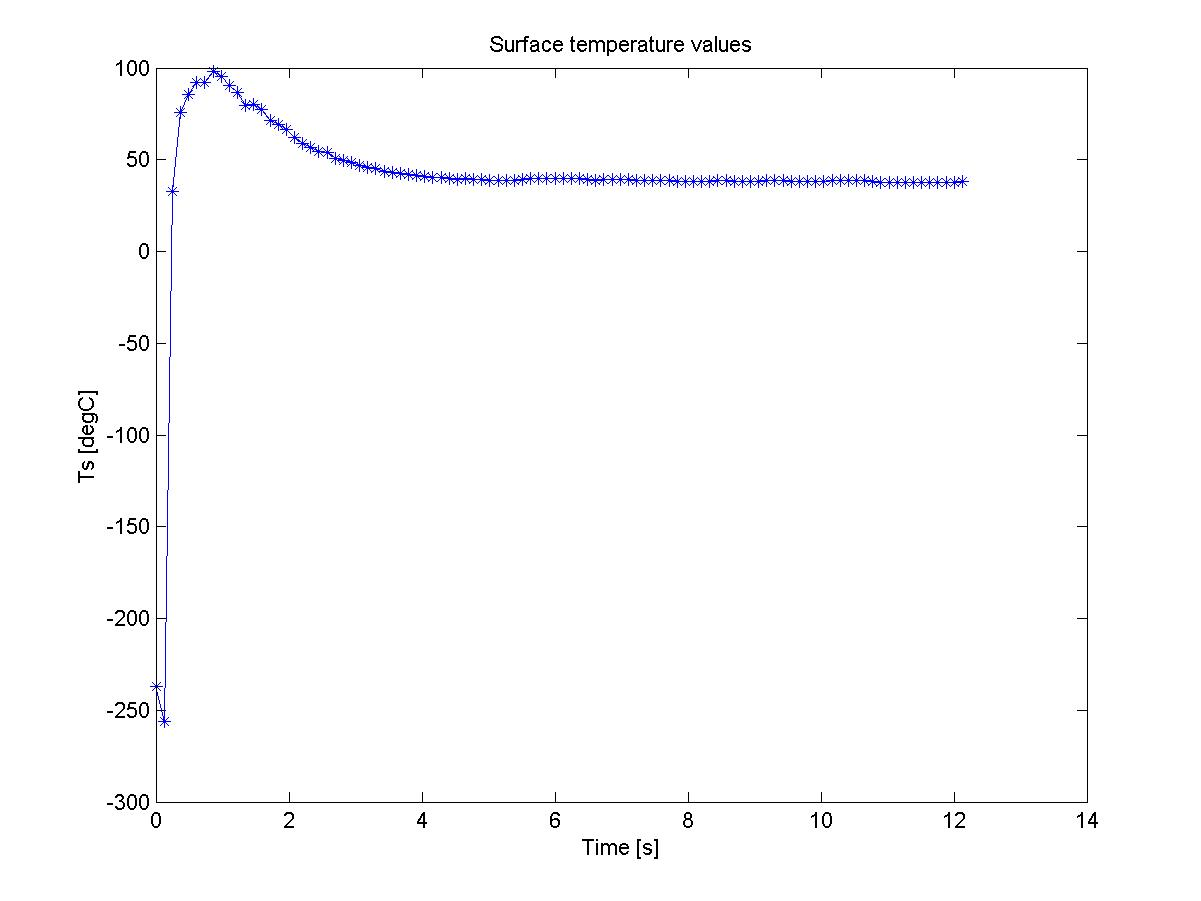
\includegraphics[width=.5\textwidth]{pics/surfaceT}
\label{fig:surfaceT}}}
\caption{(a) Heat Transfer Coefficient (b) Surface Temperature over Time}
\label{pic:surfaceT}
\end{figure}

 %!TEX root = Report.tex
\chapter{Conclusion}\label{sec:conclusion}






\section{Suitability of PIV for the measured Flow Field}
Since our flow field is quasi two dimensional and only few velocity compenents normal to the measured plane occur,  the PIV is very well suited. In addition, the Reynolds Number of the fluid is very low and therfore a laminar flow is formed. This is advantageous because in a turbulent flow information is lost. The fluctuations of the velocity that typically occur in turbulent flows can not be registered, as the flow field is divided in small panels and averaged in these panels.\\

One of the main issues in PIV is the framerate of the camera. Only with the development of CCD high speed cameras, the required frame rates are reached. As we have a very slow flow (around $0.5\ mm/s$), the framerate of the camera is hence not an issue and no expensive highspeed camera is required. \\

Due to the optics of the camera, a slight distortion at the border of the image arises. As we have exactly at the same areas the highest displacments/velocities, we need to consider this fact in our interpretation.

\section{Limitations And Possible Improvements}

As it was mentioned before, the change of quality in the pictures wasn't traceable enough with the used shutter aperture and exposure times used. Altough the good plausability of our results, a higher difference in those mentioned parameters would help us to better understand their effects on the final results. \\

The effect of peak loking could be overcome with a filtering of the images taken. An induced blurriness (for example with averaging of the sorroundings of a particle) in the images would make the particles bigger and their movement better traceable for the case of small displacements. This way, the peak locking could decrease and the histogram of displacement would look much more homogeneously distributed.

%---------------------------------------------------------------------------
% Literature

 %\cleardoublepage
 %\nocite{*}						% we want to include all entries from the bib file, even if they were not cited in the report
 %\bibliographystyle{plain}			% Style
 
 %\addcontentsline{toc}{chapter}{Bibliography}	% add bibliography to table of contents
 
 %\bibliography{bib/references}		% include bibliography
 %\cleardoublepage



%---------------------------------------------------------------------------
% Appendix

 \appendix
 %!TEX root = Report.tex
\chapter{MATLAB Code}\label{c:datasheets}


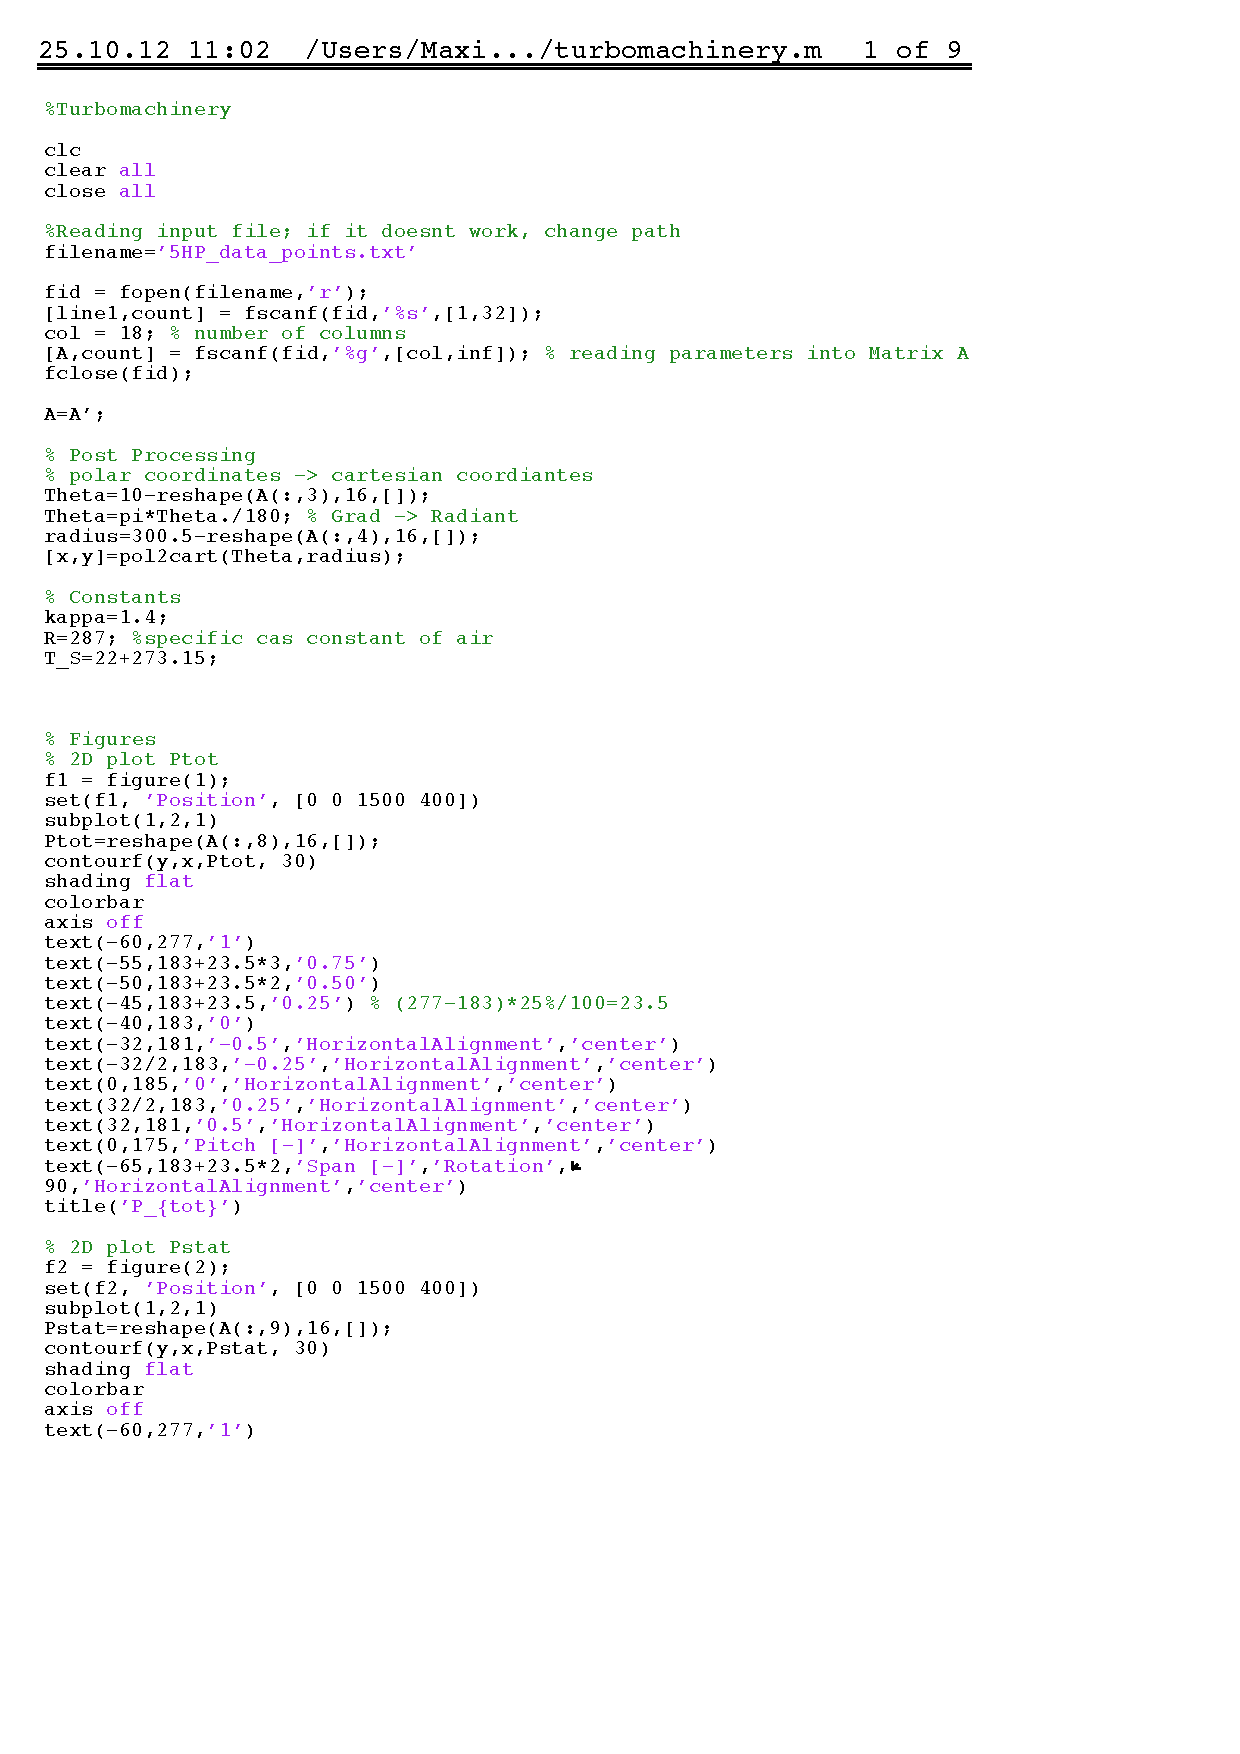
\includepdf[pages=-,frame=true, scale=0.9]{pics/code.pdf}

%\includepdf[pages={1,3,4-5},angle=0,nup=2x2,frame=true, scale=0.9]{datasheets/PicDatasheet.pdf}
%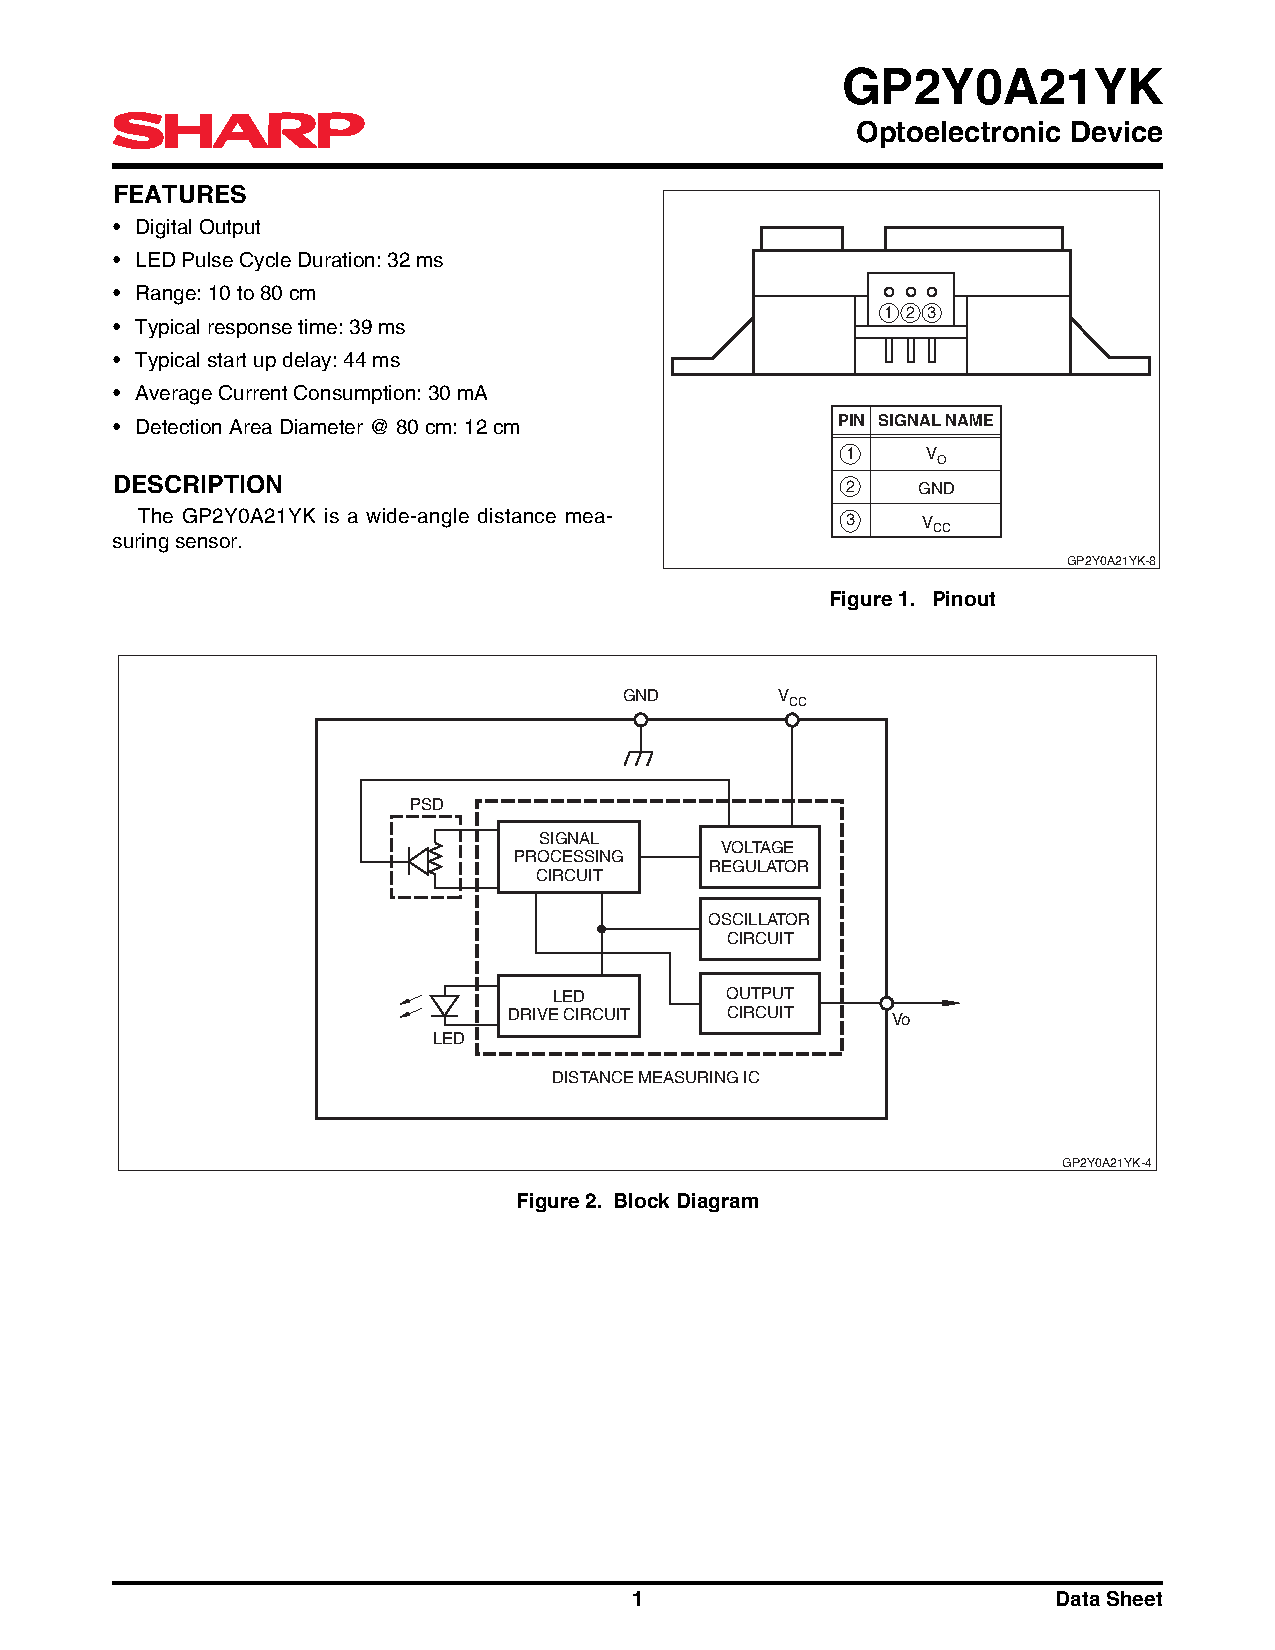
\includepdf[pages=1]{datasheets/SharpDatasheet.pdf}
%
%\cleardoublepage

%
%\chapter{Something Else}\label{sec:something}
%
%Add here some other appendix material \dots
%
% \cleardoublepage
 
 
 





%---------------------------------------------------------------------------

\end{document}
%===========================================================================
